% !TEX root = ../../book_ML.tex
\chapter{Ôn tập Đại số tuyến tính}
\label{cha:linearalgebra}

\section{Lưu ý về ký hiệu}

Trong cuốn sách này, những số vô hướng được biểu diễn bởi các chữ cái
in nghiêng và có thể viết hoa, ví dụ $x_1, N, y, k$. Các ma trận được biểu diễn
bởi các chữ viết hoa in đậm, ví dụ $\mathbf{X, Y, W} $. Các vector được biểu
diễn bởi các chữ cái thường in đậm, ví dụ $\mathbf{y}, \mathbf{x}_1 $. Nếu
không giải thích gì thêm, các vector được mặc định hiểu là các vector cột.

Đối với vector, $\mathbf{x} = [x_1, x_2, \dots, x_n]$ được hiểu là một vector
hàng, $\mathbf{x} = [x_1; x_2; \dots; x_n] $ được hiểu là vector cột. Chú ý
sự khác nhau giữa dấu phẩy ($,$) và dấu chấm phẩy ($;$). Đây chính là ký hiệu
được Matlab sử dụng. Nếu không giải thích gì thêm, một chữ cái viết thường in
đậm được hiểu là một vector cột.

Tương tự, trong ma trận, $\mathbf{X} = [\mathbf{x}_1, \mathbf{x}_2, \dots,
\mathbf{x}_n]$ được hiểu là các vector cột $\mathbf{x}_j$ được đặt cạnh nhau
theo thứ tự từ trái qua phải để tạo ra ma trận $\mathbf{X}$. Trong khi
$\mathbf{X} = [\mathbf{x}_1; \mathbf{x}_2; \dots; \mathbf{x}_m]$ được hiểu là
các vector $\mathbf{x}_i$ được đặt chồng lên nhau theo thứ tự từ trên xuống dưới
dể tạo ra ma trận $\mathbf{X}$. Các vector được ngầm hiểu là có kích thước phù
hợp để có thể xếp cạnh hoặc xếp chồng lên nhau. Phần tử ở hàng thứ $i$, cột thứ
$j$ được ký hiệu là $x_{ij}$.

% \textit{Chú ý: Một số tài liệu có sử dụng ký hiệu khác như sau. Cho một ma
% trận $\bX \in \R^{m \times n}$, cột thứ $i$ của ma trận được ký hiệu là
% $\bX_{:,i}$; hàng thứ $j$ của ma rận được ký hiệu là $\bX_{j,:}$; phần tử ở hàng
% thứ $i$, cột thứ $j$ được ký hiệu là $X_{i,j}$. Khi đọc, chúng ta cần chú ý các
% ký hiệu toán học. }

Cho một ma trận $\mathbf{W}$, nếu không giải thích gì thêm, ta hiểu rằng
$\mathbf{w}_i$ là \textbf{vector cột} thứ $i$ của ma trận đó. Chú ý sự tương ứng
giữa ký tự viết hoa và viết thường.


% section chuyen_vi (end)
% \newpage
% \index{chuyển vị}
\section{Chuyển vị và Hermitian} % (fold)
\label{sec:chuyen_vi}


% Một phép toán quan trọng trong đại số tuyến tính là \textit{chuyển vị}
% (\textit{transpose}).
\index{chuyển vị -- transpose}
\index{transpose -- chuyển vị}
Cho một ma trận/vector $\bA \in \R^{m\times n}$, ta nói $\bB \in \R^{n\times m}$ là \textit{chuyển vị} (transpose) của
$\bA$ nếu $b_{ij} = a_{ji},~\forall 1 \leq i \leq n, 1 \leq j\leq m$.

Chuyển vị của ma trận $\bA$ được ký hiệu là $\bA^T$. Cụ thể hơn:
\begin{eqnarray*}
\bx = \left[
\begin{matrix}
x_1 \\ x_2 \\ \vdots \\ x_m
\end{matrix}
\right] \Rightarrow \bx^T = \left[
\begin{matrix}
x_1 & x_2 & \dots & x_m
\end{matrix}
\right];
\end{eqnarray*}
\begin{eqnarray*}
\bA = \left[
\begin{matrix}
a_{11} & a_{12} & \dots & a_{1n} \\
a_{21} & a_{22} & \dots & a_{2n} \\
% a_{31} & a_{32} & \dots & a_{3n} \\
\dots & \dots & \ddots & \dots \\
a_{m1} & a_{m2} & \dots & a_{mn}
\end{matrix}
\right]
\Rightarrow
\bA^T = \left[
\begin{matrix}
a_{11} & a_{21}  &\dots & a_{m1} \\
a_{12} & a_{22}  & \dots & a_{m2} \\
\dots & \dots &  \ddots & \dots \\
a_{1n} & a_{2n} & \dots & a_{mn}
\end{matrix}
\right]
\end{eqnarray*}
% \begin{eqnarray}
% \bA = \left[
% \begin{matrix}
%     a_{11} & a_{12} & \dots & a_{1n} \\
%     a_{21} & a_{22} & \dots & a_{2n} \\
%     % a_{31} & a_{32} & \dots & a_{3n} \\
%     \dots & \dots & \ddots & \dots \\
%     a_{m1} & a_{m2} & \dots & a_{mn}
% \end{matrix}
% \right]
% \Rightarrow
% \bA^T = \left[
% \begin{matrix}
% a_{11} & a_{21}  &\dots & a_{m1} \\
% a_{12} & a_{22}  & \dots & a_{m2} \\
% \dots & \dots &  \ddots & \dots \\
% a_{1n} & a_{2n} & \dots & a_{mn}
% \end{matrix}
% \right]
% \end{eqnarray}
% \sec{Tích Hadamard của hai ma trận}
% \label{sec:Hamard}

Nếu $\bA \in \R^{m\times n}$ thì $\bA^T \in \R^{n\times m}$. Nếu $\bA^T = \bA$, ta
nói $\bA$ là một \textit{ma trận đối xứng}.

\index{ma trận đối xứng -- symmetric matrix}
\index{symmetric matrix -- ma trận đối xứng}
\index{Hermitian}
\index{chuyển vị liên hợp -- conjugate transpose}
\index{conjugate transpose -- chuyển vị liên hợp}
Trong trường hợp vector hay ma trận có các phần tử là số phức, việc lấy chuyển
vị thường đi kèm với việc lấy liên hợp phức. Tức là ngoài việc đổi vị trí của
các phần tử, ta còn lấy liên hợp phức của các phần tử đó. Tên gọi của phép toán
chuyển vị và lấy liên hợp này còn được gọi là \textit{chuyển vị liên hợp} (conjugate transpose), và
thường được ký hiệu bằng chữ $H$ thay cho chữ $T$. Chuyển vị liên hợp của một ma
trận $\bA$ được ký hiệu là $\bA^H$, được đọc là $\bA$ Hermitian.

Cho $\bA \in \mathbb{C}^{m\times n}$, ta nói $\bB \in \mathbb{C}^{n\times m}$ là chuyển vị liên
hợp của $\bA$ nếu
$b_{ij} = \lbar{a_{ji}},~\forall 1 \leq i \leq n, 1 \leq j \leq m$,
trong đó $\lbar{a}$ là liên hiệp phức của $a$.

\textit{Ví dụ}:
\begin{equation}
\bA = \bmt 1 + 2i &~~ & 3 - 4i \\
i &~~ & 2 \emt
\Rightarrow \bA^{H} =
\bmt 1 - 2i &~~ & -i \\
3 + 4i &~~ & 2 \emt
\end{equation}

Nếu $\bA, \bx$ là các ma trận và vector thực thì $\bA^H = \bA^T, \bx^H = \bx^T$.



Nếu chuyển vị liên hợp của một ma trận vuông phức bằng với chính nó, $\bA^H = \bA$,
ta nói ma trận đó là \textit{Hermitian}.


\section{Phép nhân hai ma trận} % (fold)
\label{sec:nhan_hai_ma_tran}
Cho hai ma trận $\bA \in \R^{m\times n}, \bB \in \R^{n \times p}$, tích của hai
ma trận được ký hiệu là $\bC = \bA\bB \in \R^{m \times p}$ trong đó phần tử ở
hàng thứ $i$, cột thứ $j$ của ma trận kết quả được tính bởi:
\begin{equation}
c_{ij} = \sum_{k=1}^na_{ik}b_{kj}, ~\forall 1\leq i \leq m, 1 \leq j \leq p
\end{equation}
Để nhân được hai ma trận, số cột của ma trận thứ nhất phải bằng số hàng của ma trận thứ hai. Trong ví dụ trên, chúng đều bằng $n$.

Giả sử kích thước các ma trận là phù hợp để các phép nhân ma trận tồn tại, ta có
một vài tính chất sau:

\begin{enumerate}

\item Phép nhân ma trận không có tính chất giao hoán. Thông thường (không
phải luôn luôn), $\bA\bB \neq \bB\bA$. Thậm chí, trong nhiều trường hợp, các
phép tính này không tồn tại vì kích thước các ma trận lệch nhau.

\item Phép nhân ma trận có tính chất kết hợp: $\bA \bB\bC = (\bA\bB)\bC = \bA(\bB\bC)$.
% \begin{equation}
% \bA \bB\bC = (\bA\bB)\bC = \bA(\bB\bC)
% \end{equation}

\item Phép nhân ma trận có tính chất phân phối đối với phép cộng: $\bA(\bB + \bC) = \bA\bB + \bA\bC$.
% \begin{equation}
%     \bA(\bB + \bC) = \bA\bB + \bA\bC
% \end{equation}

\item Chuyển vị của một tích bằng tích các chuyển vị theo thứ tự ngược lại.
Điều tương tự xảy ra với Hermitian của một tích:
\begin{equation}
(\bA\bB)^T = \bB^T \bA^T; \quad (\bA\bB)^H = \bB^H\bA^H
\end{equation}

\end{enumerate}
\index{tích vô hướng -- inner product}
\index{inner product -- tích vô hướng}
\index{trực giao -- orthogonal}
\index{orthogonal -- trực giao}
\textit{Tích trong}, hay \textit{tích vô hướng} (inner product) của hai vector $\bx, \by \in \R^n$
được định nghĩa bởi:
\begin{equation}
\bx^T\by = \by^T\bx = \sum_{i =1}^n x_iy_i
\end{equation}
Nếu tích vô hướng của hai vector khác không bằng không, ta nói hai vector đó
\textit{trực giao} (orthogonal).

Chú ý, $\bx^H\by$ và $\by^H\bx$ bằng nhau khi và chỉ khi
chúng là các số thực.

$\bx^H\bx \geq 0,~\forall\bx \in \mathbb{C}^n$ vì tích của một số phức với liên
hiệp của nó luôn là một số không âm.



Phép nhân của một ma trận $\bA \in \R^{m \times n}$ với một vector
$\bx \in \R^{n}$ là một vector $\bb \in \R^{m}$:
\begin{equation}
\bA\bx = \bb, ~\text{với} ~b_i = \bA_{i,:}\bx
\end{equation}
với $\bA_{i,:}$ là vector hàng thứ $i$ của $\bA$.

\index{phép nhân từng thành phần -- Hadamard product}
\index{Hadamard product -- phép nhân từng thành phần}
Ngoài ra, có một phép nhân khác được gọi là
\textit{phép nhân từng thành phần} hay \textit{tích Hadamard} (Hadamard product) thường xuyên được sử dụng trong machine learning. Tích Hadamard
của hai ma trận {cùng kích thước} $\bA, \bB \in \R^{m\times n}$, được ký hiệu là
$\bC = \bA \odot \bB \in \R^{m \times n}$, trong đó:
\begin{equation}
c_{ij} = a_{ij}b_{ij}
\end{equation}

\section{Ma trận đơn vị và ma trận nghịch đảo}
\label{sec:identitmatrix}
\subsection{Ma trận đơn vị} % (fold)
\label{sub:identity matrix }


\textit{Đường chéo chính} của một ma trận là tập hợp các điểm có chỉ số hàng và
cột bằng nhau. Cách định nghĩa này cũng có thể được áp dụng cho một ma trận
không vuông. Cụ thể, nếu $\bA \in \R^{m \times n}$ thì đường chéo chính của
$\bA$ bao gồm $\{a_{11}, a_{22}, \dots, a_{pp}\}$, trong đó $p = \min\{m, n\}$.

% subsection identity matrix  (end)
\index{identity matrix - ma trận đơn vị}
Một ma trận đơn vị bậc $n$ là một ma trận đặc biệt trong $\R^{n\times n}$ với
các phần tử trên đường chéo chính bằng 1, các phần tử còn lại bằng 0. Ma trận
đơn vị thường được ký hiệu là $\bI$. Khi làm việc với nhiều ma trận đơn vị với
bậc khác nhau, ta thường ký kiệu $\bI_n$ cho ma trận đơn vị bậc $n$. Dưới đây là
các ma trận đơn vị bậc 3 và bậc 4:
\begin{equation}
\bI_3 = \bmt
1 & 0 & 0 \\
0 & 1 & 0 \\
0 & 0 & 1
\emt, \quad
\bI_4 = \bmt
1 & 0 & 0 & 0\\
0 & 1 & 0 & 0 \\
0 & 0 & 1 & 0 \\
0 & 0 & 0 & 1
\emt
\end{equation}
Ma trận đơn vị có một tính chất đặc biệt trong phép nhân. Nếu $\bA \in
\R^{m\times n}$, $\bB \in \R^{n\times m}$ và $\bI$ là ma trận đơn vị bậc $n$, ta
có: $\bA\bI= \bA, \quad \bI\bB = \bB$.

Với mọi vector $\bx \in \R^n$, ta có $\bI_n \bx = \bx$.



\subsection{Ma trận nghịch đảo} % (fold)
\label{sub:inverse_matrix}
\index{inverse matrix - ma trận nghịch đảo}

Cho một ma trận vuông $\bA \in \R^{n\times n }$, nếu tồn tại một ma trận vuông
$\bB \in \R^{n\times n}$ sao cho $\bA\bB = \bI_n$, ta nói $\bA$ là \textit{khả
nghịch}, và $\bB$ được gọi là \textit{ma trận nghịch đảo} của $\bA$. Nếu không
tồn tại ma trận $\bB$ thoả mãn điều kiện trên, ta nói rằng ma trận $\bA$ là
{không khả nghịch}.

Nếu $\bA$ khả nghịch, ma trận nghịch đảo của nó được ký hiệu là $\bA^{-1}$. Ta
cũng có:
\begin{equation}
\bA^{-1}\bA = \bA\bA^{-1} = \bI
\end{equation}
% \begin{equation}
%     \bI_n \bx = \bx
% \end{equation}
Ma trận nghịch đảo thường được sử dụng để giải hệ phương trình tuyến tính. Giả
sử $\bA \in \R^{n\times n}$ là một ma trận khả nghịch và $\bb$ là một vector bất kỳ trong $\R^n$. Khi đó, phương trình:
\begin{equation}
\label{eqn:lin_eqn}
\bA\bx = \bb
\end{equation}
có nghiệm duy nhất $\bx = \bA^{-1}\bb$. Thật vậy, nhân bên trái cả hai vế của
phương trình với $\bA^{-1}$, ta có $\bA\bx = \bb \Leftrightarrow  \bA^{-1}\bA\bx = \bA^{-1}\bb \Leftrightarrow \bx = \bA^{-1}\bb$.
% \begin{equation}
%       \bA\bx = \bb \Leftrightarrow  \bA^{-1}\bA\bx = \bA^{-1}\bb \Leftrightarrow \bx = \bA^{-1}\bb
% \end{equation}

Nếu $\bA$ không khả nghịch, thậm chí không vuông, phương trình tuyến tính
\eqref{eqn:lin_eqn} có thể không có nghiệm hoặc có vô số nghiệm.

Giả sử các ma trận vuông $\bA, \bB$ là khả nghịch, khi đó tích của chúng cũng
khả nghịch, và $(\bA\bB)^{-1} = \bB^{-1}\bA^{-1}$. Quy tắc này cũng giống
với cách tính ma trận chuyển vị của tích các ma trận.
% subsection inverse_matrix (end)
% section section_name (end)

% \subsubsection{Gia nghich dao} % (fold)
% \label{ssub:gia_nghich_dao}

\section{Một vài ma trận đặc biệt khác} % (fold)
\label{sec:mot_vai_ma_tran_dac_biet_khac}

\subsection{Ma trận đường chéo} %(fold)
\label{sub:ma_tran_duong_cheo}

% \textit{Đường chéo chính} của một ma trận là tập hợp các điểm có chỉ số hàng và
% cột là như nhau. Cách định nghĩa này cũng có thể được định nghĩa cho một ma trận
% không vuông.

\index{ma trận đường chéo}

\textit{Ma trận đường chéo} là ma trận mà các thành phần khác không chỉ nằm trên
đường chéo chính. Định nghĩa này cũng có thể được áp dụng lên các ma trận không
vuông. Ma trận không (tất cả các phần tử bằng 0) và đơn vị là các ma trận đường
chéo. Một vài ví dụ về các ma trận đường chéo:% \begin{equation}
$\bmt 1 \emt, \bmt 2 & 0 \\ 0 & 0 \emt, \bmt 1 & 0 & 0 \\ 0 &2 & 0 \emt, \bmt
-1 & 0 \\ 0 & 2 \\ 0 & 0  \emt$.
% \end{equation}

Với các ma trận đường chéo vuông, thay vì viết cả ma trận, ta có thể chỉ liệt kê
các thành phần trên đường chéo chính. Ví dụ, một ma trận đường chéo vuông $\bA\in
\R^{m\times m}$ có thể được ký hiệu là $\diag(a_{11}, a_{22}, \dots, a_{mm})$
với $a_{ii}$
là phần tử hàng thứ $i$, cột thứ $i$ của ma trận $\bA$.

Tích, tổng của hai ma trận đường chéo vuông cùng bậc là một ma trận đường chéo.
Một ma trận đường chéo vuông là khả nghịch khi và chỉ khi mọi phần tử trên đường
chéo chính của nó khác không. Nghịch đảo của một ma trận đường chéo khả nghịch
cũng là một ma trận đường chéo. Cụ thể hơn, $(\diag(a_1, a_2, \dots, a_n))^{-1}
= \diag(a_1^{-1}, a_2^{-1}, \dots, a_n^{-1})$.% \begin{equation}
% (\diag(a_1, a_2, \dots, a_n))^{-1} = %\diag(\frac{1}{a_1}, \frac{1}{a_2},
% \dots, \frac{1}{a_n})
% \end{equation}

% áldfkjl

\subsection{Ma trận tam giác} % (fold)
\label{sub:ma_tran_tam_giac}
\index{ma trận tam giác}
\index{ma trận tam giác trên}
\index{ma trận tam giác dưới}

Một ma trận vuông được gọi là \textit{ma trận tam giác trên} nếu tất cả các
thành phần \textit{nằm phía dưới đường chéo chính bằng 0}. Tương tự, một ma trận
vuông được gọi là \textit{ma trận tam giác dưới} nếu tất cả các thành phần
\textit{nằm phía trên đường chéo chính bằng 0}.


Các hệ phương trình tuyến tính với ma trận hệ số ở dạng tam giác (trên hoặc
dưới) có thể được giải mà không cần tính ma trận nghịch đảo. Xét hệ:
\begin{equation}
\left\{
\begin{matrix}
a_{11}x_1 + &a_{12}x_2 + &\dots + &a_{1,n-1}x_{n-1} + & a_{1n}x_n= & b_1 \\
&a_{22}x_2 + &\dots + &a_{2, n-1}x_{n-2} + &a_{2n}x_n = & b_2 \\
&\dots  & \dots & \dots    & \dots \\
& &    &a_{n-1,n-1}x_{n-1} + &a_{n-1, n}x_n = & b_{n-1} \\
& &    & &a_{nn}x_n = & b_{n} \\
\end{matrix}
\right.
\end{equation}
Hệ này có thể được viết gọn dưới dạng $\bA\bx = \bb$ với $\bA$ là một ma trận
tam giác trên. Nhận thấy rằng phương trình này có thể giải mà không cần tính ma
trận nghịch đảo $\bA^{-1}$. Thật vậy, ta có thể giải $x_n$ dựa vào phương trình
cuối cùng. Tiếp theo, $x_{n-1}$ có thể được tìm bằng cách thay $x_n$ vào phương
trình thứ hai từ cuối. Tiếp tục quá trình này, ta sẽ có nghiệm cuối cùng $\bx$.
Quá trình giải từ cuối lên đầu và thay toàn bộ các thành phần đã tìm được vào
phương trình
\index{phép thế ngược}
hiện tại được gọi là \textit{phép thế ngược}. Nếu ma trận hệ số là một ma
\index{phép thế xuôi}
trận tam giác dưới, hệ phương trình có thể được giải bằng một quá trình ngược lại  --  lần lượt tính $x_1$ rồi $x_2, \dots, x_n$. Quá trình này được gọi là \textit{phép thế xuôi}.



\section{Định thức} % (fold)
\label{sec:dinh_thuc}
\index{định thức -- determinant}
\index{determinant -- định thức}
\subsection{Định nghĩa} % (fold)
\label{sub:dinh_nghia}

Định thức của một ma trận vuông $\bA$ được ký hiệu là $\det(\bA)$ hoặc $\det
\bA$. Có nhiều cách định nghĩa khác nhau của \textit{định thức}. Chúng ta sẽ sử
dụng cách định nghĩa dựa trên quy nạp theo bậc $n$ của ma trận.

Với $n = 1$, $\det(\bA)$ chính bằng phần tử duy nhất của ma trận đó.

Với một ma trận vuông bậc $n>1$:
\begin{equation}
\bA = \left[
\begin{matrix}
a_{11} & a_{12} & \dots & a_{1n} \\
a_{21} & a_{22} & \dots & a_{2n} \\
% a_{31} & a_{32} & \dots & a_{3n} \\
\dots & \dots & \ddots & \dots \\
a_{n1} & a_{n2} & \dots & a_{nn}
\end{matrix}
\right] \Rightarrow \det(\bA) = \sum_{j=1}^n (-1)^{i+j} a_{ij}\det(\bA_{ij})
\end{equation}
Trong đó $i$ là một số tự nhiên bất kỳ trong khoảng $[1, n]$ và $\bA_{ij}$ là
\index{phần bù đại số}
\textit{phần bù đại số của $\bA$ ứng với phần tử ở hàng $i$, cột $j$}. Phần bù
đại số này là một \textit{ma trận con} của $\bA$, nhận được từ $\bA$ bằng cách
xoá hàng thứ $i$ và cột thứ $j$ của nó. Đây chính là cách tính định thức dựa
trên cách khai triển hàng thứ $i$ của ma trận\footnote{Việc ghi nhớ định nghĩa
này không thực sự quan trọng bằng việc ta cần nhớ một vài tính chất của nó.}.

% subsection định_nghĩa (end) %

\subsection{Tính chất} % (fold)
\label{sub:tinh_chat}
% Một vài tính chất của định thức:

\begin{enumerate}

\item $\det(\bA) = \det(\bA^T)$: \textit{Một ma trận vuông bất kỳ và chuyển vị của
nó có định thức như nhau}.

\item \textit{Định thức của một ma trận đường chéo vuông bằng tích các
phần tử trên đường chéo chính}. Nói cách khác, nếu $\bA = \diag(a_1, a_2, \dots, a_n)$
thì $\det(\bA) = a_1a_2\dots a_n$.

\item \textit{Định thức của một ma trận đơn vị bằng 1.}

\item \textit{Định thức của một tích bằng tích các định thức.}
\begin{equation}
\det(\bA\bB) = \det(\bA) \det(\bB)
\end{equation}
với $\bA, \bB$ là hai ma trận vuông cùng chiều.


\item \textit{Nếu một ma trận có một hàng hoặc một cột là một vector
$\mathbf{0}$, thì định thức của nó bằng 0}.


\item \textit{Một ma trận là khả nghịch khi và chỉ khi định thức của nó
khác 0.}

% Từ đây ta cũng suy ra:

\item \textit{Nếu một ma trận khả nghịch, định thức của ma trận nghịch đảo
của nó bằng nghịch đảo định thức của nó.}
\begin{equation}
\det(\bA^{-1})    = \frac{1}{\det(\bA)} ~\text{vì}~ \det(\bA) \det(\bA^
{-1}) = \det(\bA \bA^{-1}) = \det(\bI) = 1.
\end{equation}



\end{enumerate}



% subsection tính_chất (end)
% section định_thức (end)

\section{Tổ hợp tuyến tính, không gian sinh} % (fold)
\label{sec:to_hop_tuyen_tinh_khong_gian_sinh}

\subsection{Tổ hợp tuyến tính} % (fold)
\label{sub:to_hop_tuyen_tinh}

\index{tổ hợp tuyến tính -- linear combination}
\index{linear combination -- tổ hợp tuyến tính}
\index{không gian sinh -- span space}
\index{span space -- không gian sinh}
Cho các vector khác không $\ba_1, \dots, \ba_n \in \R^m$ và các số thực $x_1,
\dots, x_n \in \R$,
vector:
\begin{equation}
\label{eqn:lin_com}
\bb = x_1\ba_1 + x_2\ba_2 + \dots + x_n \ba_n
\end{equation}
được gọi là một \textit{tổ hợp tuyến tính} của $\ba_1, \dots, \ba_n$. Xét ma
trận $\bA = [\ba_1, \ba_2, \dots, \ba_n] \in
\R^{m\times n}$ và $\bx = [x_1, x_2, \dots, x_n]^T$, biểu
thức~\eqref{eqn:lin_com} có thể được viết lại thành $\bb = \bA\bx$. Ta có thể
nói rằng $\bb$ là một tổ hợp tuyến tính các cột của $\bA$.


\index{doc@độc lập tuyến tính -- linearly independent}
\index{linearly independent -- độc lập tuyến tính}
\index{phụ thuộc tuyến tính -- linearly dependent}
\index{linearly dependent -- phụ thuộc tuyến tính}
Tập hợp các vector có thể biểu diễn được dưới dạng một tổ hợp tuyến tính
của một hệ vector được gọi là một \textit{không gian sinh} của hệ vector đó.
Không gian sinh của một hệ vector được ký hiệu là $\text{span}(\ba_1,
\dots, \ba_n)$. Nếu phương trình:
\begin{equation}
\label{eqn:lin_com0}
\mathbf{0} = x_1\ba_1 + x_2\ba_2 + \dots + x_n \ba_n
\end{equation}
\noindent có nghiệm duy nhất $x_1 = x_2 = \dots = x_n = 0$, ta nói rằng hệ $
\{\ba_1, \ba_2, \dots, \ba_n\}$ là một hệ \textit{độc lập tuyến tính}. Ngược
lại, nếu tồn tại $x_i \neq 0$ sao cho phương trình trên thoả mãn, ta nói rằng đó
là một hệ \textit{phụ thuộc tuyến tính}.


% \textbf{Một vài tính chất:}
\subsection{Tính chất} % (fold)
\label{sub:thtt_tinh_chat}


% subsubsection tinh_chat (end)

\begin{enumerate}
\item \textit{Một hệ là phụ thuộc tuyến tính khi và chỉ khi tồn tại một
vector trong hệ đó là tổ hợp tuyến tính của các vector còn lại. } Thật vậy,
giả sử phương trình~\eqref{eqn:lin_com0} có nghiệm khác không, và hệ số khác không là $x_i$, ta sẽ có:

\begin{equation}
\ba_i = \frac{-x_1}{x_i} \ba_1 + \dots + \frac{-x_{i-1}}{x_i}\ba_{i-1} +
\frac{-x_{i+1}}{x_i}\ba_{i+1} + \dots \frac{-x_n}{x_i}\ba_n
\end{equation}
tức $\ba_i$ là một tổ hợp tuyến tính của các vector còn lại. %Điều ngược lại
% không khó chứng minh.


\item \textit{Tập con khác rỗng của một hệ độc lập tuyến tính là một hệ độc
lập tuyến tính.}

% Việc này có thể dễ dàng chứng minh bằng phản chứng.


\item \textit{Các cột của một ma trận khả nghịch tạo thành một hệ độc lập
tuyến tính.}

Giả sử ma trận $\bA$ khả nghịch, phương trình $\bA\bx = \mathbf{0}$ có
nghiệm \textit{duy nhất} $\bx = \bA^{-1}\mathbf{0} = \mathbf{0}$. Vì vậy,
các cột của $\bA$ tạo thành một hệ độc lập tuyến tính.


\item \textit{Nếu $\bA$ là một ma trận cao, tức số hàng lớn hơn số cột, $m >
n$, tồn tại vector $\bb$ sao cho phương trình $\bA\bx = \bb$ vô nghiệm. }

Việc này có thể hình dung được trong không gian ba chiều. Không gian sinh
của một vector là một đường thẳng, không gian sinh của hai vector độc lập
tuyến tính là một mặt phẳng, tức chỉ biểu diễn được các vector nằm trong mặt
phẳng đó. Nói cách khác, với ít hơn ba vector, ta không thể biểu diễn được
mọi điểm trong không gian ba chiều.

Ta cũng có thể chứng minh tính chất này bằng phản chứng. Giả sử mọi vector
trong không gian $m$ chiều đều nằm trong không gian sinh của $n$ vector cột
của một ma trận $\bA$. Xét các cột của ma trận đơn vị bậc $m$. Vì mọi cột
của ma trận này đều có thể biểu diễn dưới dạng một tổ hợp tuyến tính của $n$
vector đã cho nên phương trình $\bA\bX = \bI$ có nghiệm. Nếu thêm các vector
cột bằng 0 vào $\bA$ và các vector hàng bằng 0 vào $\bX$ để được các ma trận
vuông, ta sẽ có $\bmt \bA & \mathbf{0} \emt \bmt \bX \\
\mathbf{0} \emt = \bA\bX = \bI$. Việc này chỉ ra rằng $\bmt \bA & \mathbf{0} \emt$ là
một ma trận khả nghịch. Đây là một điều vô lý vì định thức của $\bmt \bA &
\mathbf{0} \emt$ bằng 0.

\item \textit{Nếu $n > m$, $n$ vector bất kỳ trong không gian $m$
chiều tạo thành một hệ phụ thuộc tuyến tính}.

Thật vậy, giả sử $\{\ba_1, \dots, \ba_n \in \R^m\} $ là một hệ độc lập tuyến
tính với $n > m$. Khi đó tập con của nó $\{\ba_1, \dots, \ba_m\}$ cũng là
một hệ độc lập tuyến tính, suy ra $\bA = [\ba_1, \dots, \ba_m]$ là một ma
trận khả nghịch. Khi đó phương trình $\bA\bx = \ba_{m+1}$ có nghiệm $\bx =
\bA^{-1}\ba_{m+1}$. Nói cách khác, $\ba_{m+1}$ là một tổ hợp tuyến tính của
$\{\ba_1, \dots, \ba_m\}$. Điều này mâu thuẫn với giả thiết phản chứng. \dpcm

\end{enumerate}

\subsection{Cơ sở của một không gian} % (fold)
\label{sub:co_so_cua_mot_khong_gian}
% Nếu một hệ các vector
\index{cơ cở -- basic}
\index{basic -- cơ cở}
Một hệ các vector $\{\ba_1, \dots, \ba_n\}$ trong không gian vector $m$ chiều $V
= \R^m$ được gọi là một \textit{cơ sở} nếu hai điều kiện sau thoả mãn:
\begin{enumerate}
\item $V \equiv \text{span}(\ba_1, \dots, \ba_n)$
\item $\{\ba_1, \dots, \ba_n\}$ là một hệ độc lập tuyến tính.
\end{enumerate}

Khi đó, mọi vector $\bb \in V$ đều có thể biểu diễn \textit{duy nhất} dưới dạng
một tổ hợp tuyến tính của các $\ba_i$. Từ hai tính chất cuối ở Mục~\ref{sub:thtt_tinh_chat}, ta có thể suy ra rằng $m = n$.


\index{không gian range -- range space}
\index{range space -- không gian range}
\index{không gian null -- null space}
\index{null space -- không gian null}
\subsection{Range và Null space} % (fold)
\label{sub:range_va_null}
Với mỗi $\bA \in \R^{m \times n}$, có hai không gian con quan trọng ứng
với ma trận này.

% \begin{enumerate}
\textit{Range} của $\bA$, ký hiệu là $\mathcal{R}(\bA)$, được định nghĩa bởi
\begin{equation}
\mathcal{R}(\bA) = \{\by \in \R^{m} : \exists \bx \in \R^{n}, \bA\bx
=\by\}
\end{equation}
Nói cách khác, $\mathcal{R}(\bA)$ chính là không gian sinh của các cột của
$\bA$. $\mathcal{R}(\bA)$ là một không gian con của $\R^m$ với số chiều
bằng số lượng lớn nhất các cột độc lập tuyến tính của $\bA$.


\textit{Null} của $\bA$, ký hiệu là $\mathcal{N}(\bA)$, được định nghĩa bởi
\begin{equation}
\mathcal{N}(\bA) = \{\bx \in \R^n : \bA\bx = \mathbf{0}\}
\end{equation}
Mỗi vector trong $\mathcal{N}(\bA)$ tương ứng với một bộ các hệ số làm cho
tổ hợp tuyến tính các cột của $\bA$ bằng vector 0. $\mathcal{N}(\bA)$ có thể
được chứng minh là một không gian con trong $\R^n$. Khi các cột của $\bA$ là
độc lập tuyến tính, phần tử duy nhất của $\mathcal{N}(\bA)$ là $\bx = \bA^{-1}\mathbf{0} = \mathbf{0}$.

% \end{enumerate}

$\mathcal{R}(\mathbf{A})$ và $\mathcal{N}(\bA)$ là các không gian con vector
với số chiều lần lượt là $\dim(\mathcal{R}(\bA))$ và $\dim(\mathcal{N}(\bA))$,
ta có tính chất quan trọng sau đây:
\begin{equation}
\dim(\mathcal{R}(\bA)) + \dim(\mathcal{N}(\bA)) = n
\end{equation}

% \newpage
% subsection range_va_null (end)
\index{hạng -- rank}
\index{rank -- hạng}
\def\rank{\text{rank}}
\section{Hạng của ma trận} % (fold)
\label{sec:hang_cua_ma_tran}
\textit{Hạng} của một ma trận $\bA \in \R^{m \times n}$, ký hiệu là
$\rank(\bA)$, được định nghĩa là số lượng lớn nhất các cột của nó tạo thành một
hệ độc lập tuyến tính.

Dưới đây là các tính chất quan trọng của hạng.
\begin{enumerate}

\item \textit{Một ma trận có hạng bằng 0 khi và chỉ khi nó là ma trận 0}.

\item \textit{Hạng của một ma trận bằng hạng của ma trận chuyển vị.}
$$\rank(\bA) = \rank(\bA^T)$$ Nói cách khác, số lượng lớn nhất các cột
độc lập tuyến tính của một ma trận bằng với số lượng lớn nhất các hàng
độc lập tuyến tính của ma trận đó. Từ đây ta suy ra tính chất dưới đây.

\item \textit{Hạng của một ma trận không thể lớn hơn số hàng hoặc số cột
của nó.}

Nếu $\bA \in \R^{m \times n}$, thì $\rank(\bA) \leq \min(m, n)$.

\item \textit{Hạng của một tích không vượt quá hạng của mỗi ma trận nhân tử.}
$$\rank(\bA\bB) \leq \min(\rank(\bA), \rank(\bB))$$

\item \textit{Hạng của một tổng không vượt quá tổng các hạng.}
\begin{equation}
\rank(\bA + \bB) \leq \rank(\bA) + \rank(\bB)
\end{equation}
Điều này chỉ ra rằng một ma trận có hạng bằng $k$ không thể được biểu diễn dưới
dạng tổng của ít hơn $k$ ma trận có hạng bằng 1. Trong Chương~\ref{cha:svd},
chúng ta sẽ thấy rằng một ma trận có hạng bằng $k$ có thể biểu diễn được
dưới dạng đúng $k$ ma trận có hạng bằng 1. %Chúng ta sẽ gặp lại tính chất này nhiều lần nếu đi
% sâu hơn vào các thuật toán Machine Learning.


\item Bất đẳng thức Sylvester về hạng: nếu $\bA \in \R^{m\times n}, \bB \in
\R^{n \times k}$, thì $$\rank{(\bA)} + \rank{(\bB)} - n \leq \rank{(\bA\bB)}$$


\end{enumerate}
Xét một ma trận vuông $\bA \in \R^{n\times }$, hai điều kiện bất kỳ trong các điều kiện dưới đây là tương đương:
% \begin{enumerate}

%     \item $\bA$ là một ma trận khả nghịch.

%     \item $\det(\bA) \neq 0$.

%     \item Các cột của $\bA$ tạo thành một cơ sở trong không gian $n$ chiều.

%     \item $\rank(\bA) = n$

% \end{enumerate}

\begin{multicols}{2}
\begin{itemize}

\item $\bA$ là một ma trận khả nghịch.

\item Các cột của $\bA$ tạo thành một cơ sở trong không gian $n$ chiều.


\item $\det(\bA) \neq 0$.

\item $\rank(\bA) = n$
\end{itemize}
\end{multicols}

% subsubsection co_so_cua_mot_khong_gian (end)
% % Câu hỏi được đặt ra là với một vector $\bb$ và một ma trận $\bA$ bất kỳ, có bao
% % nhiêu cách biểu diễn $\bb$ như là một tổ hợp tuyến tính các cột của $\bA$?

% % Câu trả lời phụ thuộc vào việc ma trận $\bA$ có khả nghịch hay không. Nếu $\bA$
% % khả nghịch, tồn tại duy nhất một bộ các số $x_1, \dots, x_n$ thoả mãn phương
% % trình~\eqref{eqn:lin_com}, đó là $\bx = \bA^{-1}\bb$. Nếu $\bA$ không khả
% % nghịch,

% % ******************************************************************************

% % subsection tổ_hợp_tuyến_tính (end)

% \subsection{Độc lập tuyến tính} % (fold)
% \label{sub:doc_lap_tuyen_tinh}

% subsection độc_lập_tuyến_tính (end)

% subsection tổ_hợp_tuyến_tính_không_gian_sinh (end)
% subsubsection giả_nghịch_đảo (end)
% \newpage
\section{Hệ trực chuẩn, ma trận trực giao}
\label{sec:linalg_orthogonality}
\subsection{Định nghĩa} % (fold)
% \label{sub:dinh_nghia}
% \index{trực chuẩn,}
\index{cơ sở -- basic!trực giao -- orthogonal}
\index{basic -- cơ sở!orthogonal -- trực giao}
\index{cơ sở -- basic!trực chuẩn -- orthonormal}
\index{basic -- cơ sở!orthonormal -- trực chuẩn}
\index{ma trận trực giao -- orthogonal matrix}
\index{orthogonal matrix -- ma trận trực giao}

Một hệ cơ sở $\{\mathbf{u}_1, \mathbf{u}_2,\dots, \mathbf{u}_m \in
\mathbb{R}^m\}$ được gọi là \textit{trực giao} nếu mỗi vector khác không và tích
vô hướng của hai vector khác nhau bất kỳ bằng không:
\begin{equation}
\mathbf{u}_i \neq \mathbf{0}; ~~ \mathbf{u}_i^T \mathbf{u}_j = 0
~ \forall ~1 \leq i \neq j \leq m
\end{equation}
Một hệ cơ sở $\{\mathbf{u}_1, \mathbf{u}_2,\dots, \mathbf{u}_m \in
\mathbb{R}^m\}$ được gọi là \textit{trực chuẩn} nếu nó là một hệ \textit{trực
giao} và độ dài Euclid (xem thêm Mục~\ref{sub:norms}) của mỗi vector bằng 1:
\begin{eqnarray}
\label{eqn:26_4}
\mathbf{u}_i^T \mathbf{u}_j = \left\{
\begin{matrix}
1 & \text{nếu} &i = j \\\
0 & \text{nếu} &i \neq j
\end{matrix}
\right.
\end{eqnarray}
% (o.w. là cách viết ngắn gọn của \textit{trong các trường hợp còn lai} (viết tắt
% của \textit{otherwise}).)
Gọi $\mathbf{U} = [\mathbf{u}_1, \mathbf{u}_2,\dots, \mathbf{u}_m]$ với
$\{\mathbf{u}_1, \mathbf{u}_2,\dots, \mathbf{u}_m \in \mathbb{R}^m\}$ là
\textit{trực chuẩn}. Từ \eqref{eqn:26_4} ta có thể suy ra:
\begin{equation}
\label{eqn:or_matrix}
\mathbf{UU}^T = \mathbf{U}^T\mathbf{U} = \mathbf{I}
\end{equation}
trong đó $\mathbf{I}$ là ma trận đơn vị bậc $m$. Nếu một ma trận thoả mãn điều
kiện~\eqref{eqn:or_matrix}, ta gọi nó là một \textit{ma trận trực giao}.
\textit{Ma trận loại này không được gọi là ma trận trực chuẩn, không có định
nghĩa cho ma trận trực chuẩn.}

\index{ma trận unitary}

Nếu một ma trận vuông phức $\bU$ thoả mãn $\bU\bU^H = \bU^H\bU = \bI$, ta nói
rằng $\bU$ là một ma \textit{trận unitary}.
% Một vài tính chất:

\subsection{Tính chất} % (fold)

\begin{enumerate}

\item \textit{Nghịch đảo của một ma trận trực giao chính là chuyển vị của
nó.}
\begin{equation*}
\mathbf{U}^{-1} = \mathbf{U}^T
\end{equation*}
\item \textit{Nếu $\mathbf{U}$ là một ma trận trực giao thì chuyển vị của nó
$\mathbf{U}^T$ cũng là một ma trận trực giao.}
\item \textit{Định thức của một ma trận trực giao bằng $1$ hoặc $-1$.}

Điều này có thể suy ra từ việc $\det(\mathbf{U}) = \det(\mathbf{U}^T)$ và
$\det(\mathbf{U}) \det(\mathbf{U}^T) = \det(\mathbf{I}) = 1$.

\item \textit{Ma trận trực giao thể hiện cho phép xoay một vector} (xem thêm
mục~\ref{sec:doi_he_co_so}).

Giả sử có hai vector $\mathbf{x,y} \in \mathbb{R}^m$ và một ma trận trực
giao $\mathbf{U} \in \mathbb{R}^{m \times m}$. Dùng ma trận này để xoay hai
vector trên ta được $\mathbf{Ux}, \mathbf{Uy}$. Tích vô hướng của hai vector
mới là:
\begin{equation*}
(\mathbf{Ux})^T (\mathbf{Uy}) = \mathbf{x}^T \mathbf{U}^T \mathbf{Uy} = \mathbf{x}^T\mathbf{y}
\end{equation*}
như vậy \textit{phép xoay không làm thay đổi tích vô hướng giữa hai vector}.

\item Giả sử $\hat{\mathbf{U}} \in \mathbb{R}^{m \times r}, r < m$ là một ma
trận con của ma trận trực giao $\mathbf{U}$ được tạo bởi $r$ cột của
$\mathbf{U}$, ta sẽ có $\hat{\mathbf{U}}^T\hat{\mathbf{U}} =
\mathbf{I}_{r}$. Việc này có thể được suy ra từ \eqref{eqn:26_4}.

\end{enumerate}



\section{Biễu diễn vector trong các hệ cơ sở khác nhau}
\label{sec:doi_he_co_so}
Trong không gian $m$ chiều, toạ độ của mỗi điểm được xác định dựa trên một hệ
toạ độ nào đó. Ở các hệ toạ độ khác nhau, toạ độ của mỗi điểm cũng khác nhau.

Tập hợp các vector $\mathbf{e}_1, \dots, \mathbf{e}_m$ mà mỗi vector
$\mathbf{e}_i$ có đúng 1 phần tử khác 0 ở thành phần thứ $i$ và phần tử đó bằng
1, được gọi là \textit{hệ cơ sở đơn vị} (hoặc \textit{hệ đơn vị}, hoặc
\textit{hệ chính tắc}) trong không gian $m$ chiều. Nếu xếp các vector
$\mathbf{e}_i, i = 1, 2, \dots, m$ cạnh nhau theo đúng thứ tự đó, ta sẽ được ma
trận đơn vị $m$ chiều.

Mỗi vector cột $\mathbf{x} = [x_1, x_2, \dots, x_m] \in \mathbb{R}^m$ có thể coi
là một tổ hợp tuyến tính của các vector trong hệ cơ sở chính tắc:
\begin{equation}
\mathbf{x} = x_1 \mathbf{e}_1 + x_2 \mathbf{e}_2 + \dots + x_m\mathbf{e}_m
\end{equation}
% \newpage
Giả sử có một hệ cơ sở độc lập tuyến tính khác $\mathbf{u}_1, \mathbf{u}_2,
\dots, \mathbf{u}_m$. Trong hệ cơ sở mới này, $\bx$ được viết dưới dạng
\begin{equation}
\mathbf{x} = y_1 \mathbf{u}_1 + y_2 \mathbf{u}_2 + \dots + y_m\mathbf{u}_m =
\mathbf{U}\mathbf{y}
\end{equation}
với $\mathbf{U} = \bmt \bu_1 & \dots &\bu_m\emt$. Lúc này, vector $\mathbf{y} =
[y_1, y_2, \dots, y_m]^T$ chính là biểu diễn của $\mathbf{x}$ trong hệ cơ sở
mới. Biểu diễn này là duy nhất vì $\mathbf{y} =
\mathbf{U}^{-1} \mathbf{x}$.

Trong các ma trận đóng vai trò như hệ cơ sở, các ma
trận trực giao, tức $\mathbf{U}^T\mathbf{U} = \mathbf{I}$, được quan tâm nhiều
hơn vì nghịch đảo và chuyển vị của chúng bằng nhau, $\mathbf{U}^{-1} = \mathbf{U}^T$.
% \begin{equation}
%     \mathbf{U}^{-1} = \mathbf{U}^T
% \end{equation}
Khi đó, $\mathbf{y}$ có thể được tính một cách nhanh chóng $\mathbf{y} = \mathbf{U}^{T} \mathbf{x}$.
% \begin{equation}
%     \mathbf{y} = \mathbf{U}^{T} \mathbf{x}
% \end{equation}
Từ đó suy ra $y_i = \mathbf{x}^T \mathbf{u}_i = \mathbf{u}_i^T\mathbf{x}, i= 1,
\dots, m$. Dưới góc nhìn hình học, hệ trực giao tạo thành một hệ trục toạ độ
Descartes vuông góc. Hình~\ref{fig:change_basis} là một ví dụ về việc chuyển hệ
cơ sở trong không gian hai chiều.

Có thể nhận thấy rằng vector $\mathbf{0}$ được biểu diễn như nhau trong mọi hệ
cơ sở.


\begin{figure}[t]
% caption on side
\floatbox[{\capbeside\thisfloatsetup{capbesideposition={right,top},capbesidewidth=6cm}}]{figure}[\FBwidth]
{\caption{
Chuyển đổi toạ độ trong các hệ cơ sở khác nhau. Trong hệ toạ độ
$O\be_1\be_2$, $\bx$ có toạ độ là $(x_1, x_2)$. Trong hệ toạ độ
$O\bu_1\bu_2$, $\bx$ có toạ độ là $(y_2, y_2)$.
}
\label{fig:change_basis}}
{ % figure here
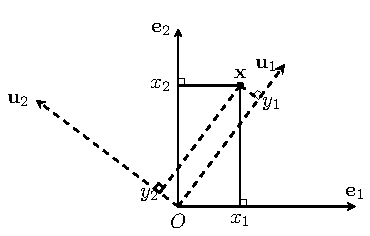
\includegraphics[width=.5\textwidth]{Chapters/07_DimemsionalityReduction/27_pca/latex/changebasis.pdf}
}
\end{figure}


Việc chuyển đổi hệ cơ sở sử dụng ma trận trực giao có thể được coi như một phép
xoay trục toạ độ. Nhìn theo một cách khác, đây cũng chính là một phép xoay
vector dữ liệu theo chiều ngược lại, nếu ta coi các trục toạ độ là cố định.
Trong Chương~\ref{cha:pca}, chúng ta sẽ thấy một ứng dụng quan trọng của
việc đổi hệ cơ sở.


% \newpage

\section{Trị riêng và vector riêng} % (fold)
\label{sec:tri_rieng_ve_vector_rieng}
\index{trị riêng -- eigenvalues}
\index{eigenvalues -- trị riêng}
\index{vector riêng -- eigenvectors}
\index{eigenvectors -- vector riêng}

\subsection{Định nghĩa} % (fold)
\label{sub:dinh_nghia}


% \def\C{\mathbb{C}}
Cho một ma trận vuông $\bA \in \mathbb{R}^{n\times n}$, một vector $\bx \in \mathbb{C}^n (\bx
\neq \mathbf{0} )$ và một số vô hướng $\lambda \in \mathbb{C}$. Nếu
% $\bA\bx = \lambda \bx$,
\begin{equation}
\bA\bx = \lambda \bx,
\end{equation}
ta nói $\lambda$ là một \textit{trị riêng} của $\bA$, $\bx$ là một \textit{vector riêng} ứng với trị riêng $\lambda$.
% và $\bx$ lần lượt là \textit{trị riêng, vector riêng} của ma trận $\bA$.

% thì ta nói rằng $\lambda$ và $\bx$ lần lượt
% là \textit{trị riêng} (\textit{eigenvalue}) và \textit{vector riêng}
% (\textit{eigenvector}) của ma trận $\bA$.


Từ định nghĩa ta cũng có $(\bA - \lambda \bI)\bx = 0$, tức $\bx$ là một vector nằm trong không gian $\mathcal{N}(\bA - \lambda \bI)$. Vì $\bx \neq 0$, ta có  $\bA - \lambda \bI$ là một ma
trận không khả nghịch. Nói cách khác $\det(\bA - \lambda \bI) = 0$, tức
$\lambda$ là nghiệm của phương trình $\det(\bA -t \bI) = 0$.
\index{da@đa thức đặc trưng -- characteristic polynomial}
\index{characteristic polynomial -- đa thức đặc trưng}
Định thức này là một đa thức bậc $n$ của $t$. Đa thức này còn được gọi là
\textit{đa thức đặc trưng} của $\bA$, được ký hiệu là $p_{\bA}(t)$. Tập hợp tất
\index{phổ của ma trận -- spectrum}
\index{spectrum -- phổ của ma trận}
cả các trị riêng của một ma trận vuông còn được gọi là \textit{phổ} của ma trận
đó.

% \subsection{Đa thức đặc trưng} % (fold)
% \label{sub:da_thuc_dac_trung}

% subsection da_thuc_dac_trung (end)

\subsection{Tính chất} % (fold)
\label{sub:tinh_chat}

% subsection tinh_chat (end)

% Định lý
% section trị_riêng_và_vector_riêng (end)



% \subsection{Trị riêng và vector riêng}
% Cho một ma trận vuông $\mathbf{A} \in \mathbb{R}^{n\times n}$, nếu số vô hướng
% $\lambda$ và vector $\mathbf{x} \neq \mathbf{0} \in \mathbb{R}^n$ thoả mãn:

% \begin{equation}
% \mathbf{Ax} = \lambda \mathbf{x}
% \end{equation}
% thì $\lambda$ được gọi là một trị riêng của $\mathbf{A}$ và $\mathbf{x}$ được gọi là vector riêng tương ứng với trị riêng đó.

% Một vài tính chất:

\def\ElA{E_{\lambda}(\bA)}
\begin{enumerate}
\item Giả sử $\lambda$ là một trị riêng của $\bA \in \mathbb{C}^{n\times n}$, đặt $\ElA$ là tập các vector riêng ứng với trị riêng $\lambda$ đó. Bạn đọc có thể chứng minh được:
\begin{itemize}
\item Nếu $\bx \in \ElA$ thì $k\bx \in \ElA, \forall k \in \mathbb{C}$.

\item Nếu $\bx_1, \bx_2 \in \ElA$ thì $\bx_1 + \bx_2 \in \ElA$.
\end{itemize}
Từ đó suy ra \textit{tập hợp các vector riêng ứng với một trị riêng của một
ma trận vuông tạo thành một không gian vector con}, thường được gọi là
\textit{không gian riêng} ứng với trị riêng đó.
\index{không gian riêng -- eigenspace}
\index{eigenspace -- không gian riêng}

\item \textit{Mọi ma trận vuông bậc $n$ đều có $n$ trị riêng, kể cả lặp và phức.}

\item \textit{Tích của tất cả các trị riêng của một ma trận bằng định thức
của ma trận đó. Tổng tất cả các trị riêng của một ma trận bằng tổng các
phần tử trên đường chéo của ma trận đó.}


\item \textit{Phổ của một ma trận bằng phổ của ma trận chuyển vị của nó.}


\item \textit{Nếu $\bA, \bB$ là các ma trận vuông cùng bậc thì
$p_{\bA\bB}(t) = p_ {\bB\bA}(t)$}. Như vậy, tuy $\bA\bB$ có thể khác
$\bB\bA$, đa thức đặc trưng của $\bA\bB$ và $\bB\bA$ luôn bằng nhau
nhau. Tức phổ của hai tích này là trùng nhau.

\item \textit{Tất cả các trị riêng của một ma trận Hermitian là các số
thực.} Thật vậy, giả sử $\lambda$ là một trị riêng của một ma trận Hermitian $\bA$ và $\bx$ là một vector riêng ứng với trị riêng đó. Từ định nghĩa ta
suy ra:
\begin{equation}
\bA\bx = \lambda\bx \Rightarrow (\bA\bx)^H = \bar{\lambda} \bx^H
\Rightarrow  \bar{\lambda}\bx^H = \bx^H\bA^H = \bx^H\bA
\end{equation}
với $\bar{\lambda}$ là liên hiệp phức của số vô hướng $\lambda$. Nhân cả hai
vế vào bên phải với $\bx$ ta có:
\begin{equation}
\bar{\lambda}\bx^H\bx = \bx^H\bA\bx = \lambda \bx^H \bx \Rightarrow
(\lambda - \bar{\lambda})\bx^H\bx = 0
\end{equation}
% Vì $\bx^H\bx$
vì $\bx \neq 0$ nên $\bx^H\bx \neq 0$. Từ đó suy ra $\bar{\lambda} =
\lambda$, tức $\lambda$ phải là một số thực.

\item Nếu $(\lambda, \bx)$ là một cặp trị riêng, vector riêng của một ma
trận khả nghịch $\bA$, thì $\displaystyle(\frac{1}{\lambda}, \bx)$ là một
cặp trị riêng, vector riêng của $\bA^{-1}$, vì $\displaystyle \bA\bx =
\lambda\bx \Rightarrow \frac{1} {\lambda}\bx = \bA^{-1}\bx$.


\end{enumerate}

%     \item Với \href{http://machinelearningcoban.com/2017/03/12/convexity/#positive-semidefinite}{\textit{ma trận xác định dương}}, tất cả
%     các trị riêng của nó đều là các số thực dương. Với \textit{ma trận nửa xác
%     định dương}, tất cả các trị riêng của nó đều là các số thực không âm.

% Tính chất cuối cùng có thể được suy ra từ định nghĩa của ma trận (nửa) xác định
% dương. Thật vậy, gọi $\mathbf{u} \neq \mathbf{0}$ là vector riêng ứng với một
% trị riêng $\lambda$ của ma trận $\mathbf{A}$ xác định dương, ta có:
% \begin{equation}
%     \mathbf{Au} = \lambda \mathbf{u} \Rightarrow \mathbf{u}^T\mathbf{Au} =
%                     \lambda \mathbf{u}^T\mathbf{u} = \lambda \|\mathbf{u}\|_2^2
% \end{equation}

% Vì $\mathbf{A}$ là nửa xác định dương nên với mọi $\mathbf{u} \neq \mathbf{0}$:
% $\mathbf{u}^T\mathbf{Au} \geq 0$; $\mathbf{u} \neq 0$ nên
% $\|\mathbf{u}\|_2^2 > 0$. Từ đó suy ra $\lambda$ là một số không âm.

\section{Chéo hoá ma trận} % (fold)
\label{sec:cheo_hoa_ma_tran}

Việc phân tích một đại lượng toán học ra thành các đại lượng nhỏ hơn mang lại
nhiều hiệu quả. Phân tích một số thành tích các thừa số nguyên tố giúp kiểm tra
một số có bao nhiêu ước số. Phân tích đa thức thành nhân tử giúp tìm nghiệm của
đa thức. Việc phân tích một ma trận thành tích của các ma trận đặc biệt cũng mang lại nhiều lợi ích trong việc giải hệ phương trình tuyến tính,
tính luỹ thừa của ma trận, xấp xỉ ma trận,... Trong mục này, chúng ta sẽ ôn
lại một phương pháp phân tích ma trận quen thuộc có tên là \textit{chéo hoá ma
trận}.

Giả sử $\bx_1, \dots, \bx_n \neq \mathbf{0}$ là các vector riêng của một ma trận
vuông $\bA$ ứng với các trị riêng lặp hoặc phức $\lambda_1, \dots, \lambda_n$:
\begin{math}
\bA\bx_i = \lambda_i \bx_i, ~\forall i = 1, \dots, n
\end{math}.

Đặt $\bLambda = \diag(\lambda_1, \lambda_2, \dots, \lambda_n)$, và
$\bX = \bmt \bx_1, \bx_2, \dots, \bx_n \emt$, ta sẽ có $\bA\bX = \bX\bLambda$.
Hơn nữa, nếu các trị riêng $\bx_1, \dots, \bx_n$ là độc lập tuyến tính, ma trận
$\bX$ là một ma trận khả nghịch. Khi đó ta có thể viết $\bA$ dưới dạng tích của
ba ma trận:
\begin{equation}
\label{eqn:eigendocomposition}
\bA = \bX\bLambda\bX^{-1}
\end{equation}
Các vector riêng $\bx_i$ thường được chọn sao cho $\bx_i^T\bx_i = 1$. Cách biểu
\index{phân tích trị riêng -- eigendecomposition}
\index{eigendecomposition -- phân tích trị riêng}
diễn một ma trận như~\eqref{eqn:eigendocomposition} được gọi là phép
\textit{phân tích trị riêng}.

\index{chéo hoá ma trận -- matrix diagonalization}
\index{matrix diagonalization -- chéo hoá ma trận}
Ma trận các trị riêng $\bLambda$ là một ma trận đường chéo. Vì vậy, cách khai
triển này cũng có tên gọi là \textit{chéo hoá ma trận}. Nếu ma trận $\bA$ có thể
phân tích được dưới dạng~\eqref{eqn:eigendocomposition}, ta nói rằng $\bA$ là
\textit{chéo hoá được}.

\subsection{Lưu ý} % (fold)
\label{sub:luu y}

% subsection luu y (end)Lưu ý
\begin{enumerate}

\item Khái niệm chéo hoá ma trận chỉ áp dụng với ma trận vuông. Vì không có
định nghĩa vector riêng hay trị riêng cho ma trận không vuông.

\item Không phải ma trận vuông nào cũng chéo hoá được. Một ma trận
vuông bậc $n$ chéo hoá được khi và chỉ khi nó có đủ $n$ vector riêng độc lập
tuyến tính.

\item Nếu một ma trận là chéo hoá được, có nhiều hơn một cách chéo hoá ma
trận đó. Chỉ cần đổi vị trí của các $\lambda_i$ và vị trí tương ứng
các cột của $\bX$, ta sẽ có một cách chéo hoá mới.

\item Nếu $\bA$ có thể viết được dưới dạng~\eqref{eqn:eigendocomposition},
khi đó các luỹ thừa có nó cũng chéo hoá được. Cụ thể:
\begin{equation}
\bA^2 = (\bX \bLambda \bX^{-1})(\bX \bLambda \bX^{-1}) =
\bX\bLambda^2\bX^{-1}; \quad \bA^k = \bX \bLambda^k \bX^{-1}, ~\forall k \in
\mathbb{N}
\end{equation}
Xin chú ý rằng nếu $\lambda$ và $\bx$ là một cặp trị riêng, vector riêng
của $\bA$, thì $\lambda^k$ và $\bx$ là một cặp  trị riêng, vector riêng
của $\bA^k$. Thật vậy, $\bA^k \bx = \bA^{k-1}(\bA\bx) = \lambda \bA^
{k-1}\bx = \dots = \lambda^k \bx$.

\item Nếu $\bA$ khả nghịch, thì $\bA^{-1} = (\bX \bLambda \bX^{-1})^{-1} =
\bX \bLambda^{-1}\bX^{-1}$.
\end{enumerate}

% section cheo_hoa_ma_tran (end)

\section{Ma trận xác định dương} % (fold)
\label{sec:ma_tran_xac_dinh_duong}
% \index{positive definite matrix}
% \index{positive definite matrix! positive semidefinite}
\index{xác định dương -- positive definite}
\index{positive definite -- xác định dương}
\index{nửa xác định dương -- positive semidefinite}
\index{positive semidefinite -- nửa xác định dương}
% Trong toán tối ưu, ma trận xác định dương đóng một vài trò rất quan trọng, đặc
% biệt là trong tối ưu lồi. Mục này chúng ta sẽ làm quen với định nghĩa và một
% vài tính chất của ma trận loại này.

\subsection{Định nghĩa} % (fold)
\label{sub:dinh_nghia}
Một ma trận đối xứng\footnote{Chú ý, tồn tại những ma trận không đối xứng thoả
mãn điều kiện~\eqref{eqn:semidefinite}. Ta sẽ không xét những ma trận này trong cuốn sách.}
% \index{xác định dương -- positive definite}
$\bA \in \R^{n\times n}$ được gọi là \textit{xác định dương} nếu:
\begin{equation}
\label{eqn:semidefinite}
\bx^T\bA\bx > 0, \forall \bx \in \R^{n}, \bx \neq \mathbf{0}.
\end{equation}
Một ma trận đối xứng $\bA \in \R^{n \times n}$ được gọi là \textit{nửa xác định
dương} nếu:
\begin{equation}
\bx^T\bA\bx \geq 0, \forall \bx \in \R^{n}, \bx \neq \mathbf{0}.
\end{equation}
Trên thực tế, ma trận nửa xác định dương được sử dụng nhiều hơn.

\index{nửa xác định âm -- negative semidefinite}
\index{negative semidefinite -- nửa xác định âm}
\index{xác định âm -- negative definite}
\index{negative definite -- xác định âm}

Ma trận \textit{xác định âm} và \textit{nửa xác định âm}  cũng được định nghĩa
tương tự.

Ký hiệu $\bA \succ 0, \succeq 0, \prec 0, \preceq 0$ lần lượt để chỉ một ma trận
là xác định dương, nửa xác định dương, xác định âm, và nửa xác định âm. Ký hiệu
$\bA \succ \bB$ cũng được dùng để chỉ ra rằng $\bA - \bB
\succ 0$.

Ví dụ, $\bA = \bmt 1 & -1 \\ -1 & 1\emt$ là nửa xác định dương vì với mọi vector
$\bx = \bmt u \\ v \emt$, ta có:
\begin{equation}
\bx^T \bA\bx = \bmt u & v \emt \bmt 1 & -1 \\ -1 & 1\emt \bmt u \\ v \emt =
u^2 + v^2 - 2uv = (u - v)^2 \geq 0, \forall u, v \in \R
\end{equation}

Mở rộng, một ma trận Hermitian $\bA \in \mathbb{C}^{n\times n}$ là xác định dương nếu
\begin{equation}
\bx^H\bA\bx > 0, \forall \bx \in \mathbb{C}^{n}, \bx \neq \mathbf{0}.
\end{equation}
Các khái niệm nửa xác định dương, xác định âm, và nửa xác định dương cũng được
định nghĩa tương tự cho các ma trận Hermitian.
\subsection{Tính chất} % (fold)
\label{sub:tinh_chat}
\begin{enumerate}

\item \textit{Mọi trị riêng của một ma trận Hermitian xác định dương đều là một số
thực dương.}  Trước hết, các trị riêng của một ma trận Hermitian là các số
thực. Để chứng minh chúng là các số thực dương, ta giả sử $\lambda$ là một
trị riêng của một ma trận xác định dương $\bA$ và $\bx \neq \mathbf{0}$ là
một vector riêng ứng với trị riêng đó. Nhân vào bên trái cả hai vế của
$\bA\bx = \lambda \bx$ với $\bx^H$ ta có:
\begin{equation}
\lambda \bx^H \bx = \bx^H \bA \bx > 0
\end{equation}
% (ở đây Hermitian được dùng để xét tổng quát cho cả trường hợp ma trận phức).
Vì $\forall \bx \neq \mathbf{0}, \bx^H\bx > 0$ nên ta phải có $\lambda > 0$. Tương
tự, ta có thể chứng minh được rằng mọi trị riêng của một ma trận
nửa xác định dương là không âm.


\item \textit{Mọi ma trận xác định dương đều khả nghịch. Hơn nữa, định thức
của nó là một số dương.}  Điều này được trực tiếp suy ra từ tính chất (a).
Nhắc lại rằng định thức của một ma trận bằng tích tất cả các trị riêng của
nó.

\index{ma trận con chính -- principal submatrix}
\index{principal submatrix -- ma trận con chính}
\index{ma trận con chính trước -- leading principal submatrix}
\index{leading principal submatrix -- ma trận con chính trước}

\def\AI{\bA_{\mathcal{I}}}
\item Tiêu chuẩn Sylvester. Trước hết, chúng ta làm quen với hai khái niệm:
\textit{ma trận con chính} và \textit{ma trận con chính trước}.

Giả sử $\bA$ là một ma trận vuông bậc $n$. Gọi $\mathcal{I}$ là một tập con
khác rỗng bất kỳ của $\{1, 2, \dots, n\}$, ký hiệu $\AI$ để chỉ một ma trận
con của $\bA$ nhận được bằng cách trích ra các hàng và cột có chỉ số nằm
trong $\mathcal{I}$ của $\bA$. Khi đó, $\AI$ được gọi là một \textit{ma trận
con chính} của $\bA$. Nếu $\mathcal{I}$ chỉ bao gồm các số tự nhiên liên
tiếp từ $1$ đến $k \leq  n$, ta nói $\AI$ là một \textit{ma trận con chính
trước} bậc $k$ của $\bA$.

Tiêu chuẩn Sylvester nói rằng: \textit{Một ma trận Hermitian là xác định dương khi và chỉ khi mọi \textbf{ma trận con chính trước} của nó là xác định dương}.

Các ma trận Hermitian nửa xác định dương cần điều kiện chặt hơn: \textit{Một
ma trận Hermitian là nửa xác định dương khi và chỉ khi mọi \textbf{ma trận
con chính} của nó là nửa xác định dương}.


% \item Tiêu chuẩn Sylvester: \textit{Một ma trận Hermitian là xác định dương
% khi và chỉ khi mọi \textit{ma trận con chính trước} của nó là dương. Một ma trận
% Hermitian là nửa xác định dương nếu mọi principal minors của nó là không
% âm}. Đây là một tiêu chuẩn để kiểm tra một ma trận Hermitian $\bA \in \R^n$
% có là (nửa) xác định dương hay không. Ở đây, \textit{leading principal
% minors} và \textit{principal minors} được định nghĩa như sau:

% \index{submatrix!principal submatrix}
% \index{submatrix!principal minor}
% \index{submatrix!leading principal minor}
% \index{submatrix!leading principal matrix}

% Gọi $\mathcal{I}$ là một tập con bất kỳ của $\{1, 2, \dots, n\}$, $\AI$ là ma
% trận con của $\bA$ nhận được bằng cách trích ra các hàng và cột có chỉ số
% nằm trong $\mathcal{I}$ của $\bA$. Khi đó, $\AI$ và $\det(\AI)$ lần lượt
% được gọi là một \textit{ma trận con chính} (\textit{principal submatrix}) và
% \textit{principal minor} của $\bA$. Nếu $\mathcal{I}$ chỉ
% bao gồm các số tự nhiên liên tiếp từ $1$ đến $k \leq  n$, ta nói $\AI$ và
% $\det(\AI)$ lần lượt là một \textit{leading principal submatrix} và
% \textit{leading principal minor} bậc $k$ của $\bA$.

\item \textit{Với mọi ma trận $\bB$ không nhất thiết vuông, ma trận $\bA = \bB^H\bB$ là nửa xác định dương}.
% \textit{$\bA = \bB^H\bB$ là nửa xác định dương với mọi ma trận $\bB$
% (không nhất thiết vuông).}
Thật vậy, với mọi vector $\bx \neq 0$ với chiều phù hợp, $\bx^H\bA\bx =
\bx^H\bB^H\bB\bx = (\bB\bx)^H(\bB\bx) \geq 0$.
\index{Phân tích Cholesky -- Cholesky decomposition}
\index{Cholesky decomposition -- Phân tích Cholesky}
\item Phân tích Cholesky: \textit{Mọi ma trận Hermitian nửa xác định dương
$\bA$ đều biểu diễn được duy nhất dưới dạng $\bA = \bL\bL^H$ với $\bL$ là
một ma trận tam giác dưới với các thành phần trên đường chéo là thực dương}.

\item \textit{Nếu $\bA$ là một ma trận nửa xác định dương thì
$\bx^T\bA\bx = 0 \Leftrightarrow \bA\bx = 0$.}

Nếu $\bA\bx = 0$, dễ thấy $\bx^T\bA\bx = 0$. Nếu $\bx^T\bA\bx = 0$, với $\by \neq \mathbf{0}$ bất kỳ có cùng kích thước với $\bx$, xét hàm số
\begin{equation}
f(\lambda) = (\bx + \lambda \by)^T\bA(\bx + \lambda\by)
\end{equation}
Hàm số này không âm với mọi $\lambda$ vì $\bA$ là một ma trận nửa xác định
dương. Đây là một tam thức bậc hai của $\lambda$:
\begin{equation}
f(\lambda) = \by^T\bA\by \lambda^2 + 2\by^T\bA\bx \lambda + \bx^T\bA\bx
= \by^T\bA\by \lambda^2 + 2\by^T\bA\bx \lambda
\end{equation}
Xét hai trường hợp:
\begin{itemize}

\item $\by^T\bA\by = 0$. Khi đó, $f(\lambda) = 2\by^T\bA\bx \lambda
\geq 0, \forall \lambda$ khi và chỉ khi $\by^T\bA\bx = 0$.

\item $\by^T\bA\by > 0$. Khi đó tam thức bậc hai $f(\lambda) \geq 0,
\forall \lambda$ xảy ra khi và chỉ khi $\Delta' = (\by^T\bA\bx)^2 \leq
0$. Điều này cũng đồng nghĩa với việc $\by^T\bA\bx = 0$
\end{itemize}
Tóm lại, $\by^T\bA\bx = 0, ~\forall \by \neq \mathbf{0}$. Điều này chỉ xảy
ra nếu $\bA\bx = 0$.  \dpcm %\hfill $\square$

\end{enumerate}
% subsection tinh_chat (end)




% Nếu dấu bằng xảy ra tại một vài $\bx \neq \mathbf{0}$, ta

% subsection dinh_nghia (end)

% \begin{mydef}{Ma trận xác định dương}
% f
% \end{mydef}

% section ma_tran_xac_dinh_duong (end)

\index{chuẩn -- norm}
\index{norm -- chuẩn}
\section{Chuẩn}
\label{sec:2_norm}
Trong không gian một chiều, khoảng cách giữa hai điểm là trị tuyệt đối của hiệu
giữa hai giá trị đó. Trong không gian hai chiều, tức mặt phẳng, chúng ta thường
dùng khoảng cách Euclid để đo khoảng cách giữa hai điểm. Khoảng cách Euclid
chính là độ dài đoạn thẳng nối hai điểm trong mặt phẳng. Đôi khi, để đi từ một
điểm này tới một điểm kia, chúng ta không thể đi bằng đường thẳng vì còn phụ
thuộc vào hình dạng đường đi nối giữa hai điểm.

Việc đo khoảng cách giữa hai điểm dữ liệu nhiều chiều rất cần thiết trong
machine learning. Đây chính là lý do khái niệm \textit{chuẩn} ({norm}) ra
đời. Để xác định khoảng cách giữa hai vector $\mathbf{y}$ và $\mathbf{z}$, người
ta thường áp dụng một hàm số lên vector hiệu $\mathbf{x = y - z}$. Hàm số này
cần có một vài tính chất đặc biệt.

% \subsection{Định nghĩa}
\begin{mydef}{Chuẩn -- Norm}
Một hàm số $f: \R^n \rightarrow \R$ được gọi là một chuẩn nếu nó thỏa mãn ba
điều kiện sau đây:
\begin{enumerate}

\item $f(\mathbf{x}) \geq 0$. Dấu bằng xảy ra $\Leftrightarrow \mathbf{x = 0} $.

\item $f(\alpha \mathbf{x}) = |\alpha| f(\mathbf{x}), ~~~\forall \alpha \in \mathbb{R}\ $

\item $f(\mathbf{x}_1) + f(\mathbf{x}_2) \geq f(\mathbf{x}_1 + \mathbf{x}_2),
~~\forall \mathbf{x}_1, \mathbf{x}_2 \in \mathbb{R}^n$

\end{enumerate}\end{mydef}

{Điều kiện a)} là dễ hiểu vì khoảng cách không thể là một số âm.
Hơn nữa, khoảng cách giữa hai điểm $\mathbf{y}$ và $\mathbf{z}$ bằng 0 khi và
chỉ khi hai điểm đó trùng nhau, tức $\mathbf{x = y - z = 0} $.

{Điều kiện b)} cũng có thể được lý giải như sau. Nếu ba điểm
$\mathbf{y, v}$ và $\mathbf{z}$ thẳng hàng, hơn nữa
$\mathbf{v - y} = \alpha (\mathbf{v - z}) $ thì khoảng cách giữa $\mathbf{v}$ và
$\mathbf{y}$ gấp $ |\alpha |$ lần khoảng cách giữa $\mathbf{v}$ và
$\mathbf{z}$.

{Điều kiện c)} chính là bất đẳng thức tam giác nếu ta coi
$\mathbf{x}_1 = \mathbf{y - w}, \mathbf{x}_2 = \mathbf{w - z} $ với
$\mathbf{w}$ là một điểm bất kỳ trong cùng không gian.



\subsection{Một số chuẩn vector thường dùng}
\label{sub:norms}
% Giả sử các vectors $\mathbf{x} = [x_1; x_2; \dots; x_n]$,
% $\mathbf{y} = [y_1; y_2; \dots; y_$.

\index{chuẩn -- norm!chuẩn $\ell_2$ -- $\ell_2$ norm}
\index{norm -- chuẩn!$\ell_2$ norm -- chuẩn $\ell_2$}
\index{chuẩn -- norm!chuẩn Euclid -- Euclidean norm}
\index{norm -- chuẩn!Euclidean norm -- chuẩn Euclid}

Độ dài Euclid của một vector $\bx \in \R^n$ chính là một chuẩn, chuẩn này
được gọi là chuẩn $\ell_2$ hoặc chuẩn Euclid:
\begin{equation}
\label{eqn:norm2}
\|\mathbf{x}\|_2 = \sqrt{x_1^2 + x_2^2 + \dots + x_n^2}
\end{equation}
Bình phương của chuẩn $\ell_2$ chính là tích vô hướng của một vector với chính nó,
$\|\mathbf{x}\|_2^2 = \bx^T\bx$.
\index{chuẩn -- norm!chuẩn $\ell_p$}
\index{norm -- chuẩn!chuẩn $\ell_p$}

\newpage Với $p$ {là một số không nhỏ hơn 1} bất kỳ, hàm số:
\begin{equation}
\label{eqn:normp}
\|\mathbf{x}\|_p = (|x_1|^p + |x_2|^p + \dots |x_n|^p)^{\frac{1}{p}}
\end{equation}
được chứng minh thỏa mãn ba điều kiện của chuẩn, và được gọi là {chuẩn $\ell_p$}.
    

% Nhận thấy rằng khi $p \rightarrow 0 $ thì biểu thức \eqref{eqn:normp} trở thành
% \textit{số các phần tử khác 0 của} $\mathbf{x}$. Hàm số \eqref{eqn:normp} khi
% $p = 0$ được gọi là giả chuẩn (pseudo-norm) 0. Nó không phải là norm vì nó không
% thỏa mãn điều kiện 2 và 3 của norm. Giả chuẩn này, thường được ký hiệu là
% $\|\mathbf{x}\|_0$, chính là số lượng thành phần khác không của $\mathbf{x}$.
% Giả chuẩn này khá quan trọng trong Machine Learning vì trong nhiều bài toán,
% chúng ta cần có ràng buộc “sparse”, tức số lượng thành phần khác không của
% $\mathbf{x}$ là nhỏ.


% ******************************************************************************
\begin{figure}[t]
% caption on side
\floatbox[{\capbeside\thisfloatsetup{capbesideposition={right,top},
capbesidewidth=6.5cm}}]{figure}[\FBwidth]
{%\caption{
\caption{Minh họa chuẩn $\ell_1$ và chuẩn $\ell_2$ trong không gian hai chiều.
Chuẩn $\ell_2$ chính
là khoảng cách Euclid. Trong khi đó chuẩn $\ell_1$ là quãng
đường ngắn nhất giữa hai điểm nếu chỉ được đi theo các đường song song với
các trục toạ độ.}
\label{fig:norm12}}
{ % figure here
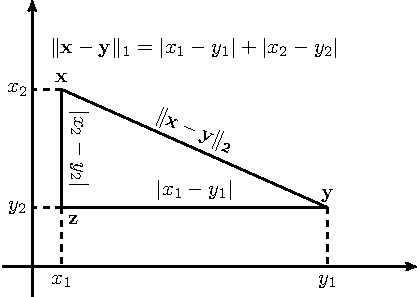
\includegraphics[width=.5\textwidth]{Chapters/02_LinearAlgebra/linearalgebra/norm12.pdf}
}
\end{figure}
% ******************************************************************************
Dưới đây là một vài giá trị của $p$ thường được dùng.
\begin{enumerate}
\item Khi $p = 2$, ta có chuẩn $\ell_2$ như ở trên.

\index{chuẩn -- norm!chuẩn $\ell_1$}
\index{norm -- chuẩn!chuẩn $\ell_1$}
\item Khi $p = 1$, ta có chuẩn $\ell_1$:
$\|\mathbf{x}\|_1 = |x_1| + |x_2| + \dots +|x_n|$ là tổng các trị tuyệt đối
của từng phần tử của $\mathbf{x}$. Hình \ref{fig:norm12} là một ví dụ  sánh
chuẩn $\ell_1$ và chuẩn $\ell_2$ trong không gian hai chiều. Chuẩn $\ell_2$
chính là khoảng cách Euclid giữa $\mathbf{x} $ và
$\mathbf{y}$. Trong khi đó, khoảng cách chuẩn $\ell_1$ giữa hai điểm này
(đường gấp khúc $\bx\bz\by$) có thể diễn giải như là quãng đường từ $\mathbf{x}
$ tới $\mathbf{y}$ nếu chỉ được phép đi song song với các trục toạ độ.

\item Khi $p \rightarrow \infty $, giả sử
$i = \arg\max_{j=1, 2, \dots, n} |x_j|$. Khi đó:
\begin{equation}
\|\bx\|_p = |x_i|\left(1 + \left|\frac{x_1}{x_i}\right|^p +
\dots +
\left|\frac{x_{i-1}}{x_i}\right|^p + \left|\frac{x_{i+1}}{x_i}\right|^p
+ \dots +\left|\frac{x_{n}}{x_i}\right|^p\right)^{\frac{1}
{p}}
\end{equation}
Ta thấy rằng
\begin{equation}
\lim_{p \rightarrow \infty}\left(1 + \left|\frac{x_1}{x_i}\right|^p +
\dots +
\left|\frac{x_{i-1}}{x_i}\right|^p + \left|\frac{x_{i+1}}{x_i}\right|^p
+ \dots +\left|\frac{x_{n}}{x_i}\right|^p\right)^{\frac{1}{p}} = 1
\end{equation}
vì đại lượng trong dấu ngoặc đơn không vượt quá $n$. Ta có
\begin{equation}
\|\bx\|_{\infty} \triangleq \lim_{p \rightarrow \infty} \|\bx\|_{p} =
|x_i| = \max_{j=1, 2, \dots, n} | x_j|
\end{equation}

\end{enumerate}

\subsection{Chuẩn Frobenius của ma trận}
\index{chuẩn -- norm!chuẩn Frobenius -- Frobenius norm}
\index{norm -- chuẩn!Frobenius norm -- chuẩn Frobenius}
Với một ma trận $\mathbf{A} \in \mathbb{R}^{m\times n}$, chuẩn thường được dùng
nhất là chuẩn Frobenius, ký hiệu là $\|\mathbf{A}\|_F$, là căn bậc hai của tổng
bình phương tất cả các phần tử của nó:
\begin{equation*}
\|\mathbf{A}\|_F = \sqrt{\sum_{i = 1}^m \sum_{j = 1}^n a_{ij}^2}
\end{equation*}
Chú ý rằng chuẩn $\ell_2$, $\|\bA\|_2$, là một chuẩn khác của ma trận, không phổ biến bằng
chuẩn Frobenius. Bạn đọc có thể xem chuẩn $\ell_2$ của ma trận trong Phụ lục~\ref{apd:lagrange}.
% \subsection{Norm 2 của ma trận}

% Chúng ta vẫn thường nhắc nhiều đến  \href{http://machinelearningcoban.com/math
% /#-norms-chuan}{norm cho vector}  nhưng chưa thực sự làm việc nhiều với norm của
% ma trận (ngoài  \href{http://machinelearningcoban.com/math/#chuan-cua-ma-
% tran}{Frobenius norm}). Trong mục này, chúng ta sẽ làm quen với 1 lớp các norm
% cho ma trận được định nghĩa dựa trên norm của vector. Lớp các norms này còn được
% gọi là \textit{Induced Norms}.

% Giả sử hàm số $\|\mathbf{x}\|_{\alpha}$ là một norm bất kỳ của vector
% $\mathbf{x}$. Ứng với norm này, định nghĩa norm tương ứng cho ma trận
% $\mathbf{A}$:
% \begin{equation}
% \|\mathbf{A}\|_{\alpha} = \max_{\mathbf{x}} \frac{\|\mathbf{Ax}\|_{\alpha}}{\|\mathbf{x}\|_{\alpha}}
% \end{equation}

% chú ý rằng ma trận $\mathbf{A}$ có thể không vuông và số cột của nó bằng với số
% chiều của $\mathbf{x}$. Như vậy, bản thân việc tính toán norm của ma trận là
% việc giải một bài toán tối ưu. Chú ý rằng hàm tối ưu có cả tử số và mẫu số là
% các norm trên vectors.

% Chúng ta sẽ quan m nhiều hơn tới chuẩn $\ell_2$. Norm 2 của ma trận được định nghĩa là:
% \begin{equation}
% \label{eqn:27_1}
% \|\mathbf{A}\|_2 = \max_{\mathbf{x}} \frac{\|\mathbf{Ax}\|_2}{\|\mathbf{x}\|_2}
% \end{equation}

% Nhận thấy rằng nếu $\mathbf{x}$ là nghiệm của bài toán tối ưu \eqref{eqn:27_1}
% thì $k\mathbf{x}$ cũng là nghiệm với $k$ là một số thực khác không bất kỳ. Không
% mất tính tổng quát, ta có thể giả sử mẫu số bằng 1. Khi đó, bài toán tối ưu
% \eqref{eqn:27_1} có thể được viết dưới dạng:
% \begin{equation}
%     \label{eqn:27_2}
%     \|\mathbf{A}\|_2 = \max_{\|\mathbf{x}\|_2 = 1} \|\mathbf{Ax}\|_2
% \end{equation}
% Nói cách khác, ta cần đi tìm $\mathbf{x}$ sao cho:
% \begin{equation}
% \label{eqn:27_3}
% \begin{aligned}
% \mathbf{x} &= \text{argmax}_{\mathbf{x}} \|\mathbf{Ax}\|_2^2  \\\
% \text{s.t.: } & \|\mathbf{x}\|_2^2 = 1
% \end{aligned}
% \end{equatn}
% Ở đây, các chuẩn $\ell_2$ đã được bình phương lên để tránh dấu căn bậc hai. Bài toán
% \eqref{eqn:27_3} có thể được giải bằng
% \href{http://machinelearningcoban.com/2017/04/02/duality/# -- phuong-phap-nhan-tu-lagrange}{Phương pháp nhân tử Lagrange}
% vì ràng buộc là một phương trình.

% Lagrangian của Bài toán \eqref{eqn:27_3} là:
% \begin{equation}
% \mathcal{L}(\mathbf{x}, \lambda) = \|\mathbf{Ax}\|_2^2 + \lambda (1 - \|\mathbf{x}\|_2^2)
% \end{equation}

% Nghiệm của bài toán \eqref{eqn:27_3} sẽ thoả mãn hệ phương trình:
% \begin{eqnarray}
%     \label{eqn:27_4}
%     \frac{\partial \mathcal{L}}{\partial \mathbf{x}} &=& 2\mathbf{A}^T\mathbf{Ax} - 2\lambda \mathbf{x} = \mathbf{0} \\\
%     \label{eqn:27_5}
%     \frac{\partial \mathcal{L}}{\partial \lambda} &=& 1 - \|\mathbf{x}\|_2^2 = 0
% \end{eqnarray}

% Từ \eqref{eqn:27_4} ta có:
% \begin{equation}
%     \label{eqn:27_6}
%     \mathbf{A}^T\mathbf{Ax} = \lambda\mathbf{x}
% \end{equation}
% Điều này suy ra rằng $\lambda$ là một trị riêng của $\mathbf{A}^T\mathbf{A}$ và $\mathbf{x}$ là 1 vector riêng ứng với trị riêng đó. Tiếp tục nhân hai vế của \eqref{eqn:27_6} với $\mathbf{x}^T$ vào bên trái, ta có:
% \begin{equation}
% \mathbf{x}^T\mathbf{A}^T\mathbf{Ax} = \lambda \mathbf{x}^T\mathbf{x} = \lambda
% \end{equation}
% Nhận thấy rằng vế trái chính là $\|\mathbf{Ax}\|_2^2$ chính là hàm mục tiêu
% trong \eqref{eqn:27_3}. Vậy hàm mục tiêu đạt giá trị lớn nhất khi $\lambda$
% đạt giá trị lớn nhất. Nói cách khác, $\lambda$ chính là trị riêng lớn nhất của
% $\mathbf{A}^T\mathbf{A}$ hay chính là \href{http://machinelearningcoban.com/2017/06/07/svd/#-nguon-goc-ten-goi-singular-value-decomposition}{singular value} lớn
% nhất của ma trận $\mathbf}$.

% Như vậy, chuẩn $\ell_2$ của một ma trận chính là singular value lớn nhất của ma trận đó.
% Và nghiệm của bài toán \eqref{eqn:27_3} chính một là \textit{right-singular
% vector} ứng với singular value đó.

% Với lý luận tương tự, chúng ta có thể suy ra rằng bài toán:
% \begin{equation}
%     \min_{\|\mathbf{x}\|_2 =1} \mathbf{x}^T\mathbf{A}^T\mathbf{A}\mathbf{x}
% \end{equation}

% có nghiệm là vector riêng ứng với trị riêng nhỏ nhất của
% $\mathbf{A}^T\mathbf{A}$. Khi đó, hàm số đạt giá trị nhỏ nhất bằng chính trị
% riêng nhỏ nhất này.


\section{Vết}
\index{vết -- trace}
\index{trace -- vết}
\textit{Vết} (trace) của một ma trận vuông $\bA$ được ký hiệu là $\trace(\bA)$, là tổng
tất cả các phần tử trên đường chéo chính của nó. Hàm vết xác định trên tập các
ma trận vuông được sử dụng nhiều trong tối ưu vì nó có những tính chất đẹp.

Các tính chất quan trọng của hàm vết, với giả sử rằng các ma trận trong hàm
vết là vuông và các phép nhân ma trận thực hiện được:
\begin{enumerate}
\item \textit{Một ma trận vuông bất kỳ và chuyển vị của nó có vết bằng
nhau}: $\trace(\bA) = \trace(\bA^T)$. Việc này được suy ra từ việc phép
chuyển vị không làm thay đổi các phần tử trên đường chéo chính của một ma
trận.


\item \textit{Vết của một tổng bằng tổng các vết}:
$$\displaystyle\trace(\sum_{i=1}^k \bA_i) = \sum_{i=1}^k \trace(\bA_i)$$

\item $\trace(k\mathbf{A}) = k\trace(\mathbf{A})$ với $k$ là một
số vô hướng bất kỳ.

\item $\trace(\mathbf{A}) = \sum_{i = 1}^D \lambda_i $ với
$\mathbf{A}$ là một ma trận vuông và $\lambda_i, i = 1, 2, \dots, N$ là toàn
bộ các trị riêng của nó, có thể lặp hoặc phức. Việc chứng minh tính chất này
có thể được dựa trên ma trận đặc trưng của $\mathbf{A}$ và định lý Viète.

\item $\trace(\mathbf{AB}) = \trace(\mathbf{BA})$. Đẳng thức này
được suy ra từ việc đa thức đặc trưng của $\bA\bB$ và $\bB\bA$ là như nhau.
Bạn đọc cũng có thể chứng minh bằng cách tính trực tiếp các phần tử trên
đường chéo chính của $\bA\bB$ và $\bB\bA$.

\item $\trace(\bA\bB\bC) = \trace(\bB\bC\bA)$, nhưng $\trace(\bA\bB\bC)$
không đồng nhất với $\trace(\bA\bC\bB)$.

\item Nếu $\bX$ là một ma trận khả nghịch cùng chiều với $\bA$ thì
\begin{equation*}
\trace (\bX\bA\bX^{-1}) = \trace(\bX^{-1}\bX\bA) = \trace(\bA)
\end{equation*}
\item $\|\mathbf{A}\|_F^2 = \trace(\mathbf{A}^T\mathbf{A}) =
\trace(\mathbf{A}\mathbf{A}^T)$ với $\mathbf{A}$ là một ma trận bất kỳ. Từ
đây ta cũng suy ra $\trace(\bA\bA^T) \geq 0$ với mọi ma trận $\bA$.

\end{enumerate}
